\documentclass[12pt,a4paper]{article}
\usepackage[utf8]{inputenc}
\usepackage{amsmath}
\usepackage{amsfonts}
\usepackage{amssymb}
\usepackage[brazil]{babel}
\usepackage{indentfirst}
\usepackage{url}
\usepackage{float}
\usepackage{color}
%%%%%%%%%%Codigos para o JAVA%%%%%%%%%%%%%%%%%%%%%%%%%%%%%%%%
\definecolor{pblue}{rgb}{0.13,0.13,1}
\definecolor{pgreen}{rgb}{0,0.5,0}
\definecolor{pred}{rgb}{0.9,0,0}
\definecolor{pgrey}{rgb}{0.46,0.45,0.48}
\usepackage{listings}
\lstset{language=Java,
  showspaces=false,
  showtabs=false,
  breaklines=true,
  showstringspaces=false,
  breakatwhitespace=true,
  commentstyle=\color{pgreen},
  keywordstyle=\color{pblue},
  stringstyle=\color{pred},
  basicstyle=\ttfamily,
  moredelim=[il][\textcolor{pgrey}]{\$\$},
  moredelim=[is][\textcolor{pgrey}]{\%\%}{\%\%}
}
%%%%%%%%%%%%%%%%%%%%%%%%%%%%%%%%Fim codigo JAVA%%%%%%%%%%%%%%
%%%%%%%%%%%Codigo geral%%%%%%%%%%%%%%%%%%%%%%%%%%%%%%%%%%%%%%
\definecolor{mygreen}{rgb}{0,0.6,0}
\definecolor{mygray}{rgb}{0.5,0.5,0.5}
\definecolor{mymauve}{rgb}{0.58,0,0.82}
\lstset{ %
  backgroundcolor=\color{white},   % choose the background color; you must add \usepackage{color} or \usepackage{xcolor}; should come as last argument
  basicstyle=\footnotesize,        % the size of the fonts that are used for the code
  breakatwhitespace=false,         % sets if automatic breaks should only happen at whitespace
  breaklines=true,                 % sets automatic line breaking
  captionpos=b,                    % sets the caption-position to bottom
  commentstyle=\color{mygreen},    % comment style
  deletekeywords={...},            % if you want to delete keywords from the given language
  escapeinside={\%*}{*)},          % if you want to add LaTeX within your code
  extendedchars=true,              % lets you use non-ASCII characters; for 8-bits encodings only, does not work with UTF-8
  frame=single,                    % adds a frame around the code
  keepspaces=true,                 % keeps spaces in text, useful for keeping indentation of code (possibly needs columns=flexible)
  keywordstyle=\color{blue},       % keyword style
  language=Octave,                 % the language of the code
  morekeywords={*,...},            % if you want to add more keywords to the set
  numbers=left,                    % where to put the line-numbers; possible values are (none, left, right)
  numbersep=5pt,                   % how far the line-numbers are from the code
  numberstyle=\tiny\color{mygray}, % the style that is used for the line-numbers
  rulecolor=\color{black},         % if not set, the frame-color may be changed on line-breaks within not-black text (e.g. comments (green here))
  showspaces=false,                % show spaces everywhere adding particular underscores; it overrides 'showstringspaces'
  showstringspaces=false,          % underline spaces within strings only
  showtabs=false,                  % show tabs within strings adding particular underscores
  stepnumber=1,                    % the step between two line-numbers. If it's 1, each line will be numbered
  stringstyle=\color{mymauve},     % string literal style
  tabsize=2,                       % sets default tabsize to 2 spaces
  title=\lstname                   % show the filename of files included with \lstinputlisting; also try caption instead of title
}
%%%%%%%%%%%%%%%%%%%%%%%%%%%%%%%%Fim codigo geral%%%%%%%%%%%%%
\RequirePackage{graphicx}
\title{JDBC com transações}
\author{Daniel Moreira Cardoso \and Gusttavo Nunes Gomes\and Jeferson Rossini Ferreira Lourenço\and Paulo Henrique Rodrigues Araujo\and Warley Rodrigues de Andrade}
 
\usepackage[left=3cm,right=3cm,top=2cm,bottom=2cm]{geometry}
\begin{document}
\begin{titlepage}
\begin{center}
\begin{figure}[htb]
                
                \label{figura:LogoIF}
        
                \centering
                \includegraphics[width=6cm]{recursos/imagens/logo.png} 
\end{figure}
Instituto Federal Goiano - Campus Ceres\\
Bacharelado em Sistemas de Informação\\
Prof. Me. Ronneesley Moura Teles\\\vspace{1cm}
Daniel Moreira Cardoso \\
Gusttavo Nunes Gomes\\
Jeferson Rossini Ferreira Lourenço\\
Paulo Henrique Rodrigues Araujo\\
Warley Rodrigues de Andrade\\
\vspace{6.0cm}
\textit{\textbf{\Large{JDBC com transações}}}\\\vspace{11cm}
Novembro\\
2017\\
\end{center}
\end{titlepage}
\tableofcontents
\newpage
\begin{center}
\textbf{\Large{JDBC com transações}}\\\vspace{0.5cm}
\end{center}
\section{Introdução}
A linguagem de programação Java, diferente de linguagens como PHP, não suporta o acesso a banco de dados diretamente, para isso ele usa uma API (conjunto de classes e interfaces) para fazer o serviço. A JDBC (Java Database Connectivity), faz o envio de instruções para qualquer banco de dados relacional, desde que haja um driver que corresponda ao mesmo presente. 
Muitos podem encontrar uma certa semelhança entre JDBC e ODBC; estão absolutamente corretos, podemos dizer a “grosso modo” que as duas seguem a mesma ideia. Ambas funcionam como meio de comunicação Banco X Aplicação, porém, ODBC é uma aplicação Windows restrito apenas a ele, enquanto a JDBC, por ser escrita em java, é multiplataforma.[1]
\section{O que é JDBC? }
\textit{Java Database Connectivy} (JDBC) é um API (Conjunto de classes e interfaces) que permite a comunicação da linguagem JAVA com qualquer banco de dados relacional. Porém é necessário um driver específico para cada SGBD.  [2]
\section{Tipos de JDBC}
Existem quatro tipos de drivers JDBC:

\begin{enumerate}
\item Tipo restrito a plataforma Windows. Esse tipo utiliza uma ODBC para se conectar com um banco de dados. Todas as chamadas ao JDBC s”ao traduzidas para chamadas ODBC (Open DataBase Connectivity);

\item O driver JDBC faz chamadas a algum outro código normalmente escrito em C.  Tanto o primeiro quando o segundo necessita de um software extra junto a sua aplicação Java;

\item Converte a chamada JDBC para uma chamada de rede. Nesta tecnologia, temos um servidor provendo a conexão com o banco de dados. Todo o código é escrito em Java;

\item Natividade 100\%, ou seja, todas as chamadas JDBC são convertidas diretamente para o protocolo de comunicação do banco de dados, ou seja, acontece um acesso direto ao DBMS.[3]

\end{enumerate}

\section{O que é transação? }
Transação é o nome que é dado à unidade de trabalho (dentro de um procedimento ou função) única, lógica e indivisível dentro de um SGBD. O código da transação é criado e disponibilizado dentro de um procedimento ou uma função: se o processamento não for realizado de forma completa ele será totalmente cancelado. Isto é feito para manter a consistência dos dados e das operações dentro do banco. [4]

Um bom exemplo de transação é a transferência bancária entre contas. Onde o valor é debitado da conta de um cliente e depois adicionado na conta de outro. 
Para fazer esta transação é muito simples, conforme o código abaixo:
\begin{center}
\begin{tabular}{|c|c|c|}
\hline 
id & nome & saldo \\ 
\hline 
1 & Daniel & 900 \\ 
\hline 
2 & Paulo & 200 \\ 
\hline 
\end{tabular} 
\end{center}
 \lstinputlisting[language=JAVA]{recursos/codigo/01.sql}
 
 
Para a transação ocorrer os dois comandos devem ser válidos, se a transação for válida os dados são enviados ao banco de dados (\textit{commit}). Caso não seja válida, ou se algo der errado o procedimento deve ser abortado (rollback). 

Quando se fala em \textit{commit} e \textit{rollback} é importante falar de autocommit, que permite que as operações sejam commitadas automaticamente. A maioria dos SGBDS usam por modo padrão o \textit{Autocommit}, ou seja, quando são executados comandos de UPDATE, INSERT ou DELETE sem iniciar uma transação explícita, essas operações são commitadas de forma automática.
%\newpage
        
\begin{figure}[h!]
	\centering
	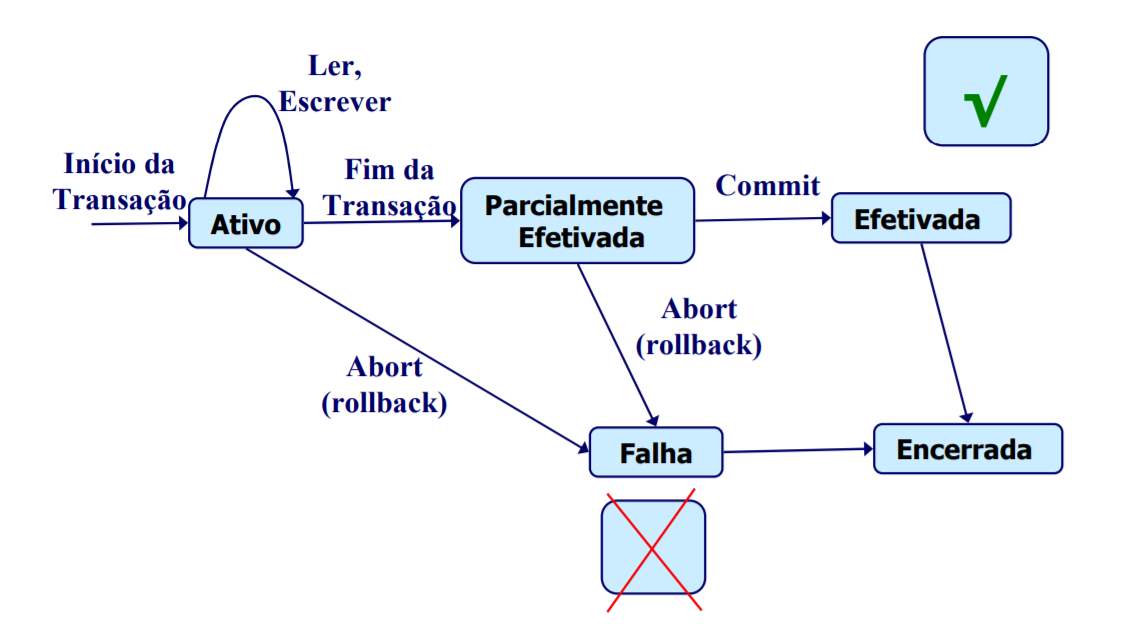
\includegraphics[width=15cm]{recursos/imagens/commit_rollback.png}
	\label{4}
	\caption{Fonte: https://www.ime.usp.br/~jef/TransacoesControleConcorrencia.pdf}
\end{figure} 

Porém as transações normalmente são feitas a nível de programação e não a nível de banco de dados (\textit{procedures}) para maior facilidade caso seja necessário migrar a base de dados para um outro SGBD. 
Agora que já vimos o que é o JDBC e transações, vamos entender como fazer transações com JDBC.
Para fazer commit com java basta chamar o método commit() da interface connection.

\begin{lstlisting}
	connection.commit();
\end{lstlisting}
O método rollback também está na interface connection
\begin{lstlisting}
	connection.rollback();
\end{lstlisting}

O auto commit também pode ser feito em java e permite gerenciar automaticamente se será feito o commit, basta no início do método chamar o método passando como argumento um valor lógico (true ou false);

\begin{lstlisting}
connection.SetAutoCommit(true);
\end{lstlisting}

Então vejamos um exemplo bastante genérico de uma transação em JAVA:
\lstinputlisting[language=JAVA]{recursos/codigo/02.java}
 
Implementando um exemplo com uma estrutura de controle.
\lstinputlisting[language=JAVA]{recursos/codigo/03.java}
%\lstinputlisting[language=Python, firstline=37, lastline=45]{source_filename.py}

\section{Driver do JDBC}
O processamento de transações é um requisito obrigatório de todos os aplicativos que desejam garantir consistência de seus dados persistentes e o uso de drivers tal como o Microsoft JDBC Driver para SQL Server que possibilita o processamento de transações pode ser realizado localmente ou distribuído. [7]

O \textit{Microsoft JDBC Driver} para SQL Server é um driver compatível com o Java Database Connectivity (JDBC) 4.2 que fornece acesso eficiente a dados para o SQL Server 2016, SQL Server 2014, SQL Server 2012, SQL Server 2008 R2, SQL Server 2008 e banco de dados do SQL Azure. [8]

O driver foi testado com os principais servidores de aplicativos, como \textit{IBM WebSphere} e \textit{SAP NetWeaver}. O driver está disponível sem custo adicional para o Windows, Mac, Red Hat e Ubuntu no GitHub da Microsoft (\url{https://github.com/microsoft/mssql-jdbc}) ou em seu próprio site. [9]


\newpage
\section{Referências Bibliográfica}
\noindent \textbf{[1]} \url {http://www.linhadecodigo.com.br/artigo/1711/java-acesso-a-dados-usando-jdbc.aspx}\\\vspace{0.2cm}

\noindent \textbf{[2] }\url{https://pt.wikipedia.org/wiki/JDBC}\\\vspace{0.2cm}

\noindent \textbf{[3]} \url {https://jmmwrite.wordpress.com/2009/08/12/diferencas-entre-as-versoes-do-jdbc/}\\\vspace{0.2cm}

\noindent\textbf{[4]} REVISTABW. Transações em Bancos de Dados.Revista Brasileira de Web: Tecnologia. Disponível em: $<$\url{http://www.revistabw.com.br/revistabw/transacoes-em-bancos-de-dados/}. Criado em: 03/01/2013. Última atualização: 24/07/2015. Visitado em: 31/10/2017 \\\vspace{0.2cm}

\noindent\textbf{[5]} \url{https://www.devmedia.com.br/aprendendo-java-com-jdbc/29116}\\\vspace{0.2cm}

\noindent\textbf{[6]} \url{http://www.guj.com.br/t/transacoes-em-java/29674} \\\vspace{0.2cm}

\noindent\textbf{[7]} \url{https://docs.microsoft.com/pt-br/sql/connect/jdbc/performing-transactions-with-the-jdbc-driver} \\\vspace{0.2cm}

\noindent\textbf{[8]} \url{https://docs.microsoft.com/pt-br/sql/connect/jdbc/microsoft-jdbc-driver-for-sql-server}\\\vspace{0.2cm}

\noindent\textbf{[9]} \url{https://github.com/microsoft/mssql-jdbc}
\end{document}
%Modelo de código para inserir figura
%\begin{figure}[h]
%\centering
%\includegraphics[width=15cm]{logo.png}
%\label{4}
%\caption{Fonte:http://...; Acesso em 06/11/2017}
%\end{figure}